\chapter{\texorpdfstring{\FEI}{FEI} signal probability for specific channels of \texorpdfstring{\B}{B}}\label{sec:appendix_fei_signal_probabilities}

In general, \FEI signal probability cannot be a good quantity for a quantitative evaluation of reconstruction quality because different classifier chains are necessary to reconstruct \Bp and \Bz candidates.
This is discussed for the comparison between \feiBp and \feiBz modes in \Cref{sec:reconstruction_overview}.
However, even for specific channels for a given $B$ modes \feiProb is not a well-calibrated quantity.
This is shown in \Cref{fig:feisigprobs1,fig:feisigprobs2} for \Bp modes and \Cref{fig:feisigprobs3,fig:feisigprobs4} for \Bz modes.
Evidently, different distributions have strongly differing shapes, which translate to different selection efficiency and/or purity.
Therefore, a general selection on \feiProb will necessary result in a direct bias to the 
selected tag-side modes and may not necessarily correspond to the `best' reconstructed mode.

\begin{figure}[htbp!]

    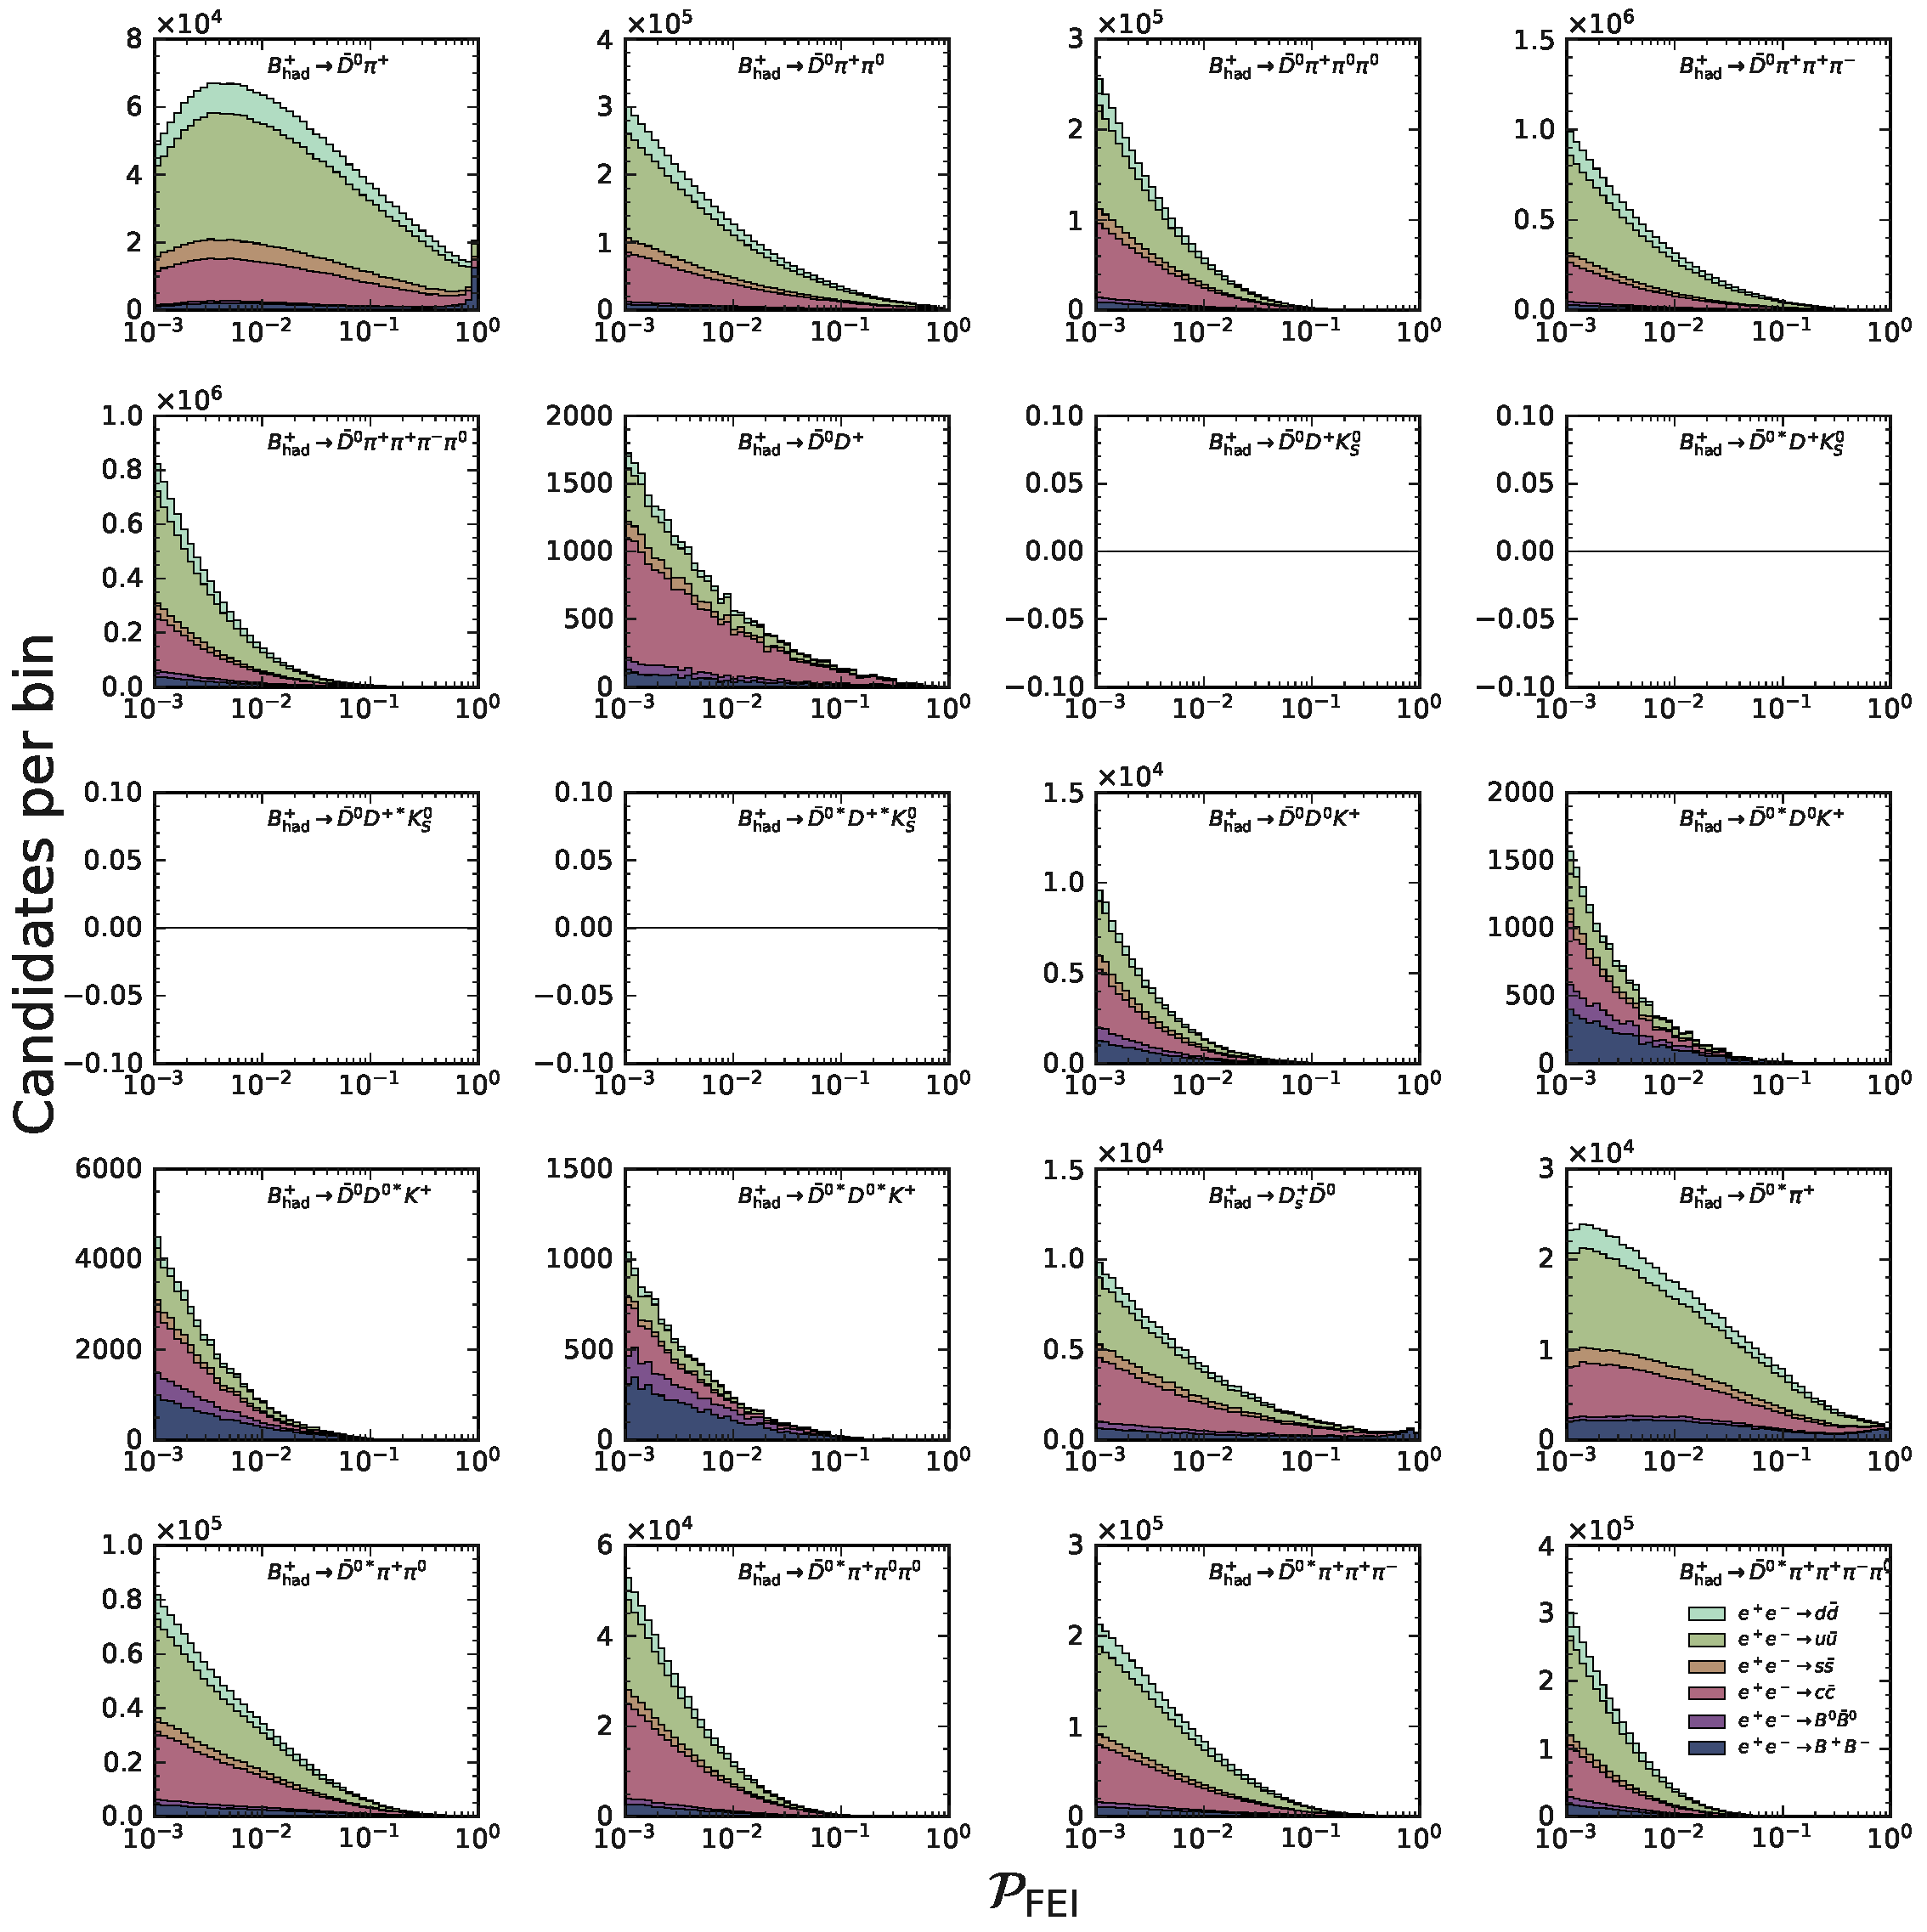
\includegraphics[width=1\textwidth]{figures/appendices/FEI_signal_probabilities/Bp_feiSigProbs1.pdf}

    \caption{\label{fig:feisigprobs1} \FEI signal probabilities for specific modes of \Bp reconstruction after requirements described in \Cref{sec:event_reconstruction}.
    This shows the signal probabilities for the first 20 \Bp modes in \Cref{tab:fei_modes}.
    Some figures are empty because no modes are reconstructed in those channels (either due to insufficient statistics, or no training available for said modes.)
    The legend, y and x axes are shared among all plots.
    }
\end{figure}

\begin{figure}[htbp!]

    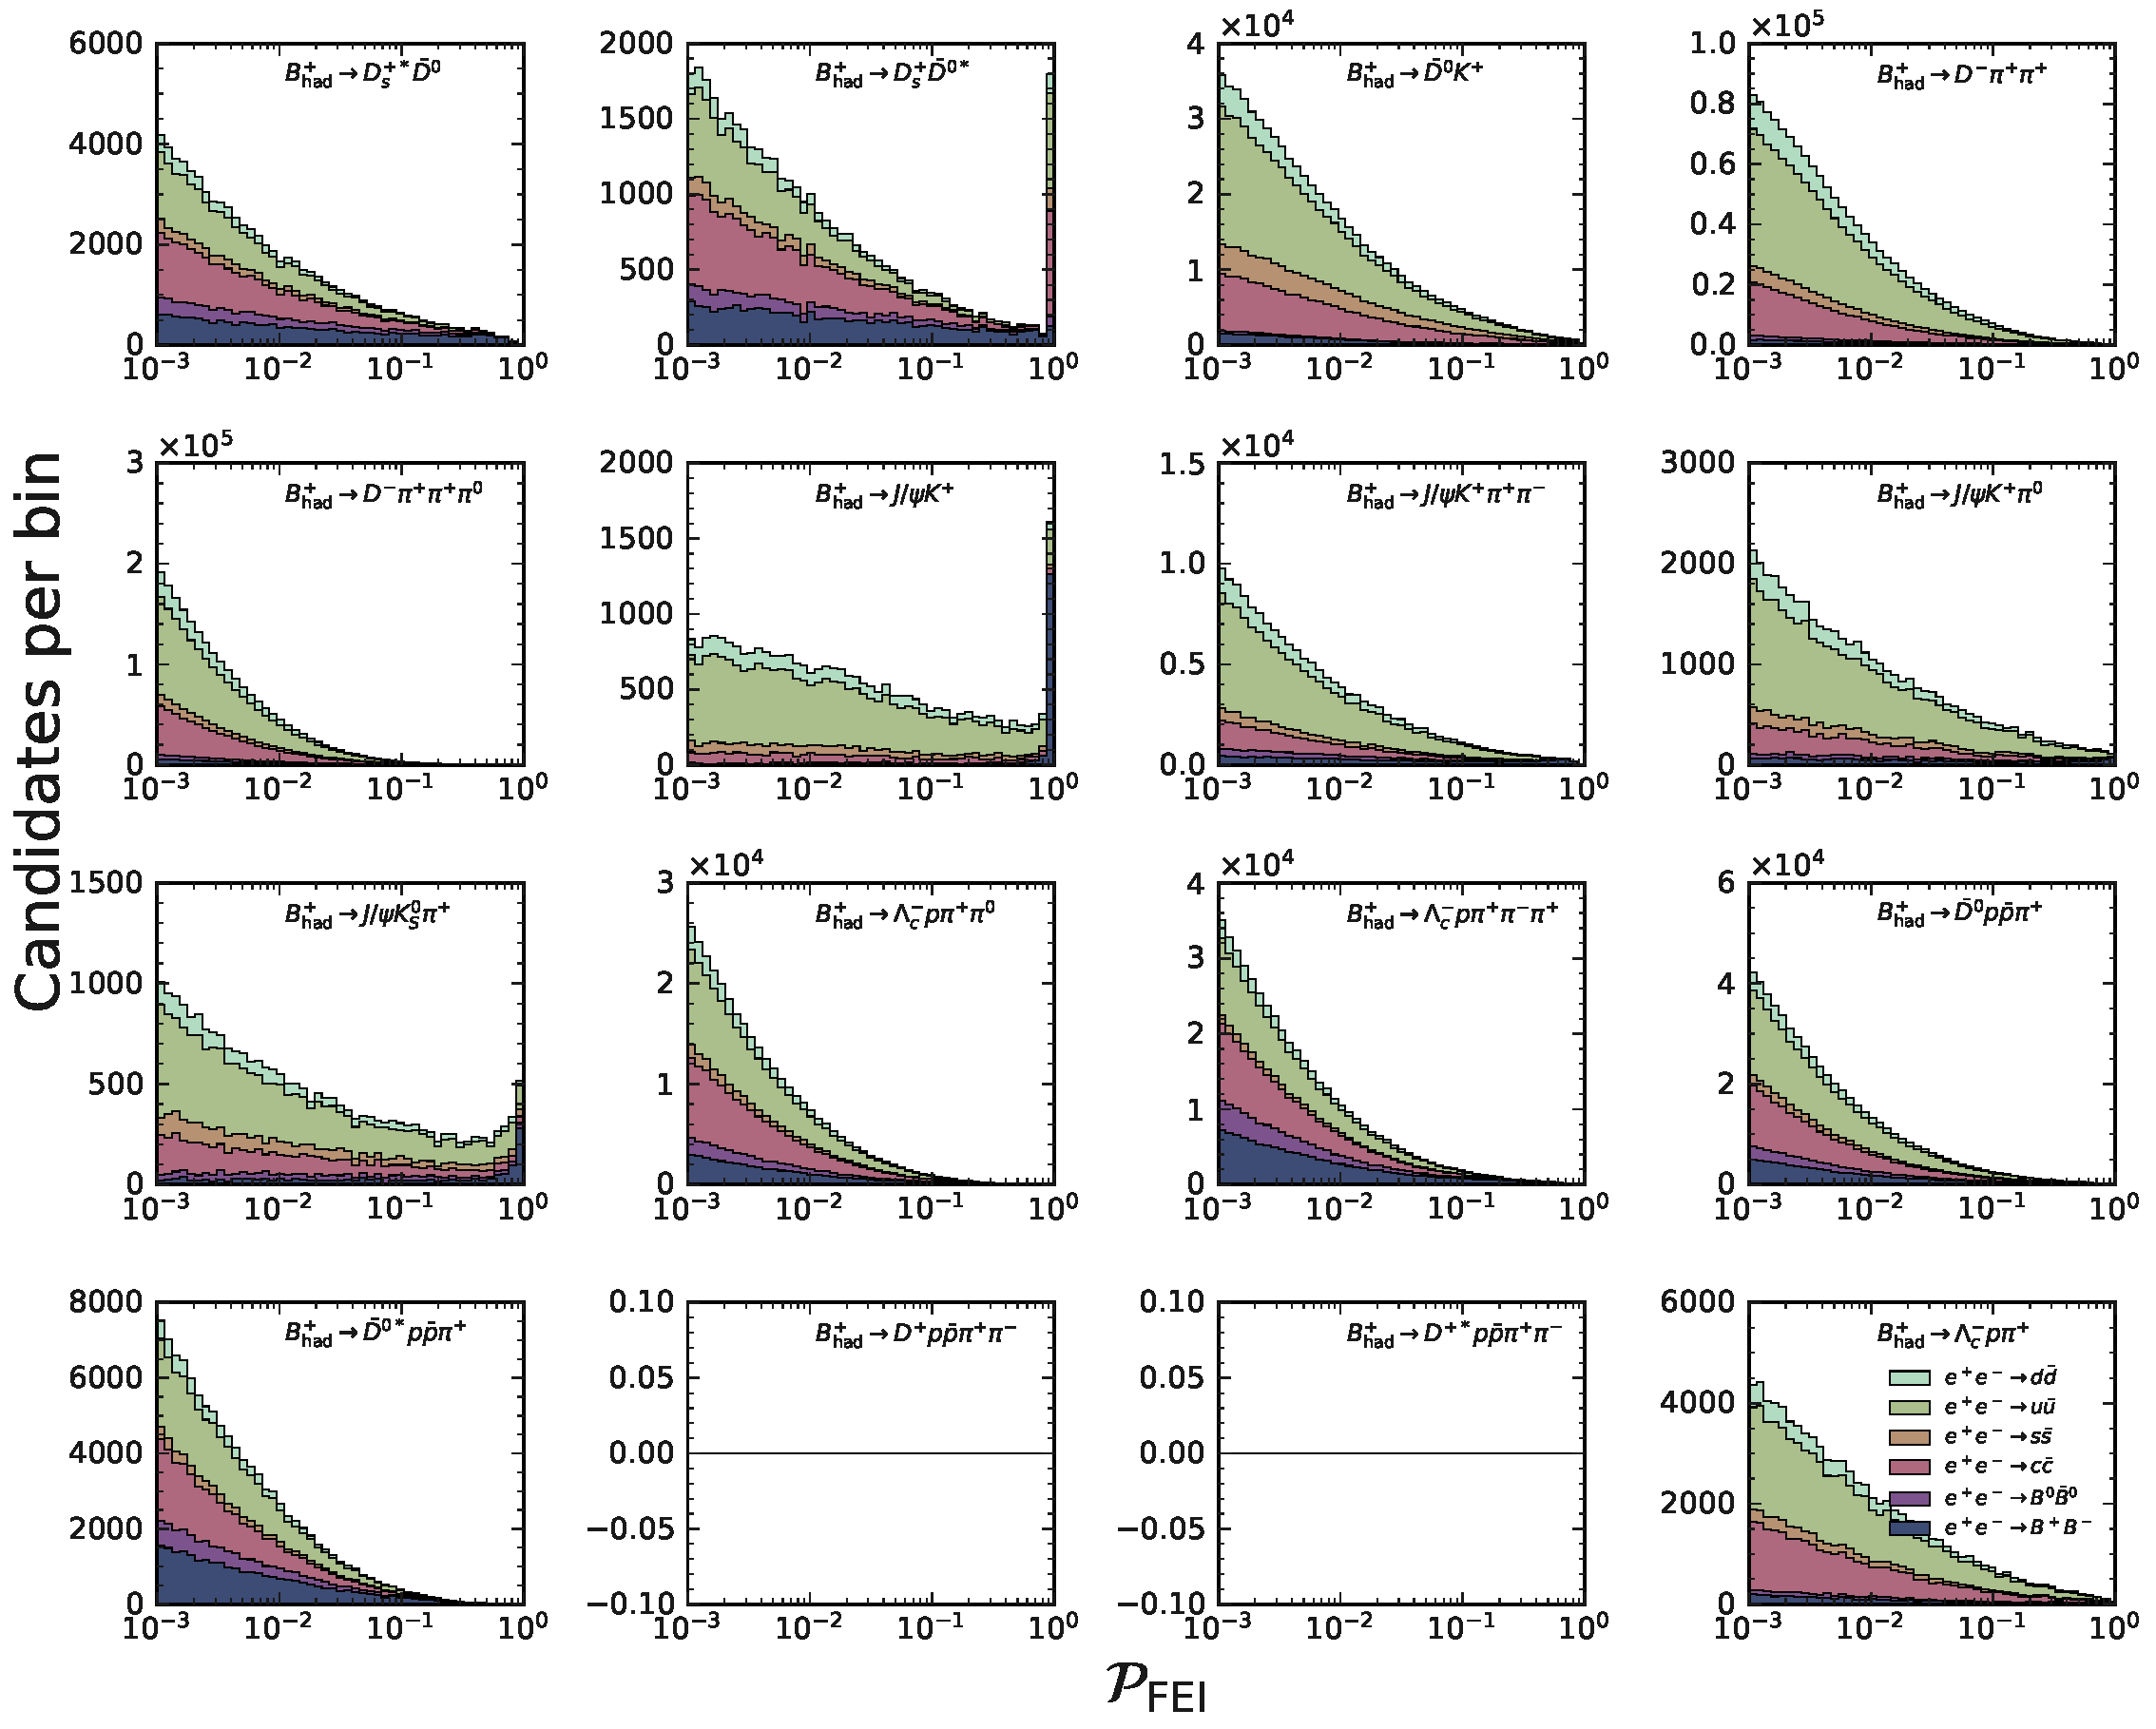
\includegraphics[width=1\textwidth]{figures/appendices/FEI_signal_probabilities/Bp_feiSigProbs2.pdf}

    \caption{\label{fig:feisigprobs2} \FEI signal probabilities for specific modes of \Bp reconstruction after requirements described in \Cref{sec:event_reconstruction}.
    This shows the signal probabilities for the modes 20-36 \Bp modes in \Cref{tab:fei_modes}.
    Some figures are empty because no modes are reconstructed in those channels (either due to insufficient statistics, or no training available for said modes.)
    The legend, y and x axes are shared among all plots.
    }
\end{figure}

\begin{figure}[htbp!]

    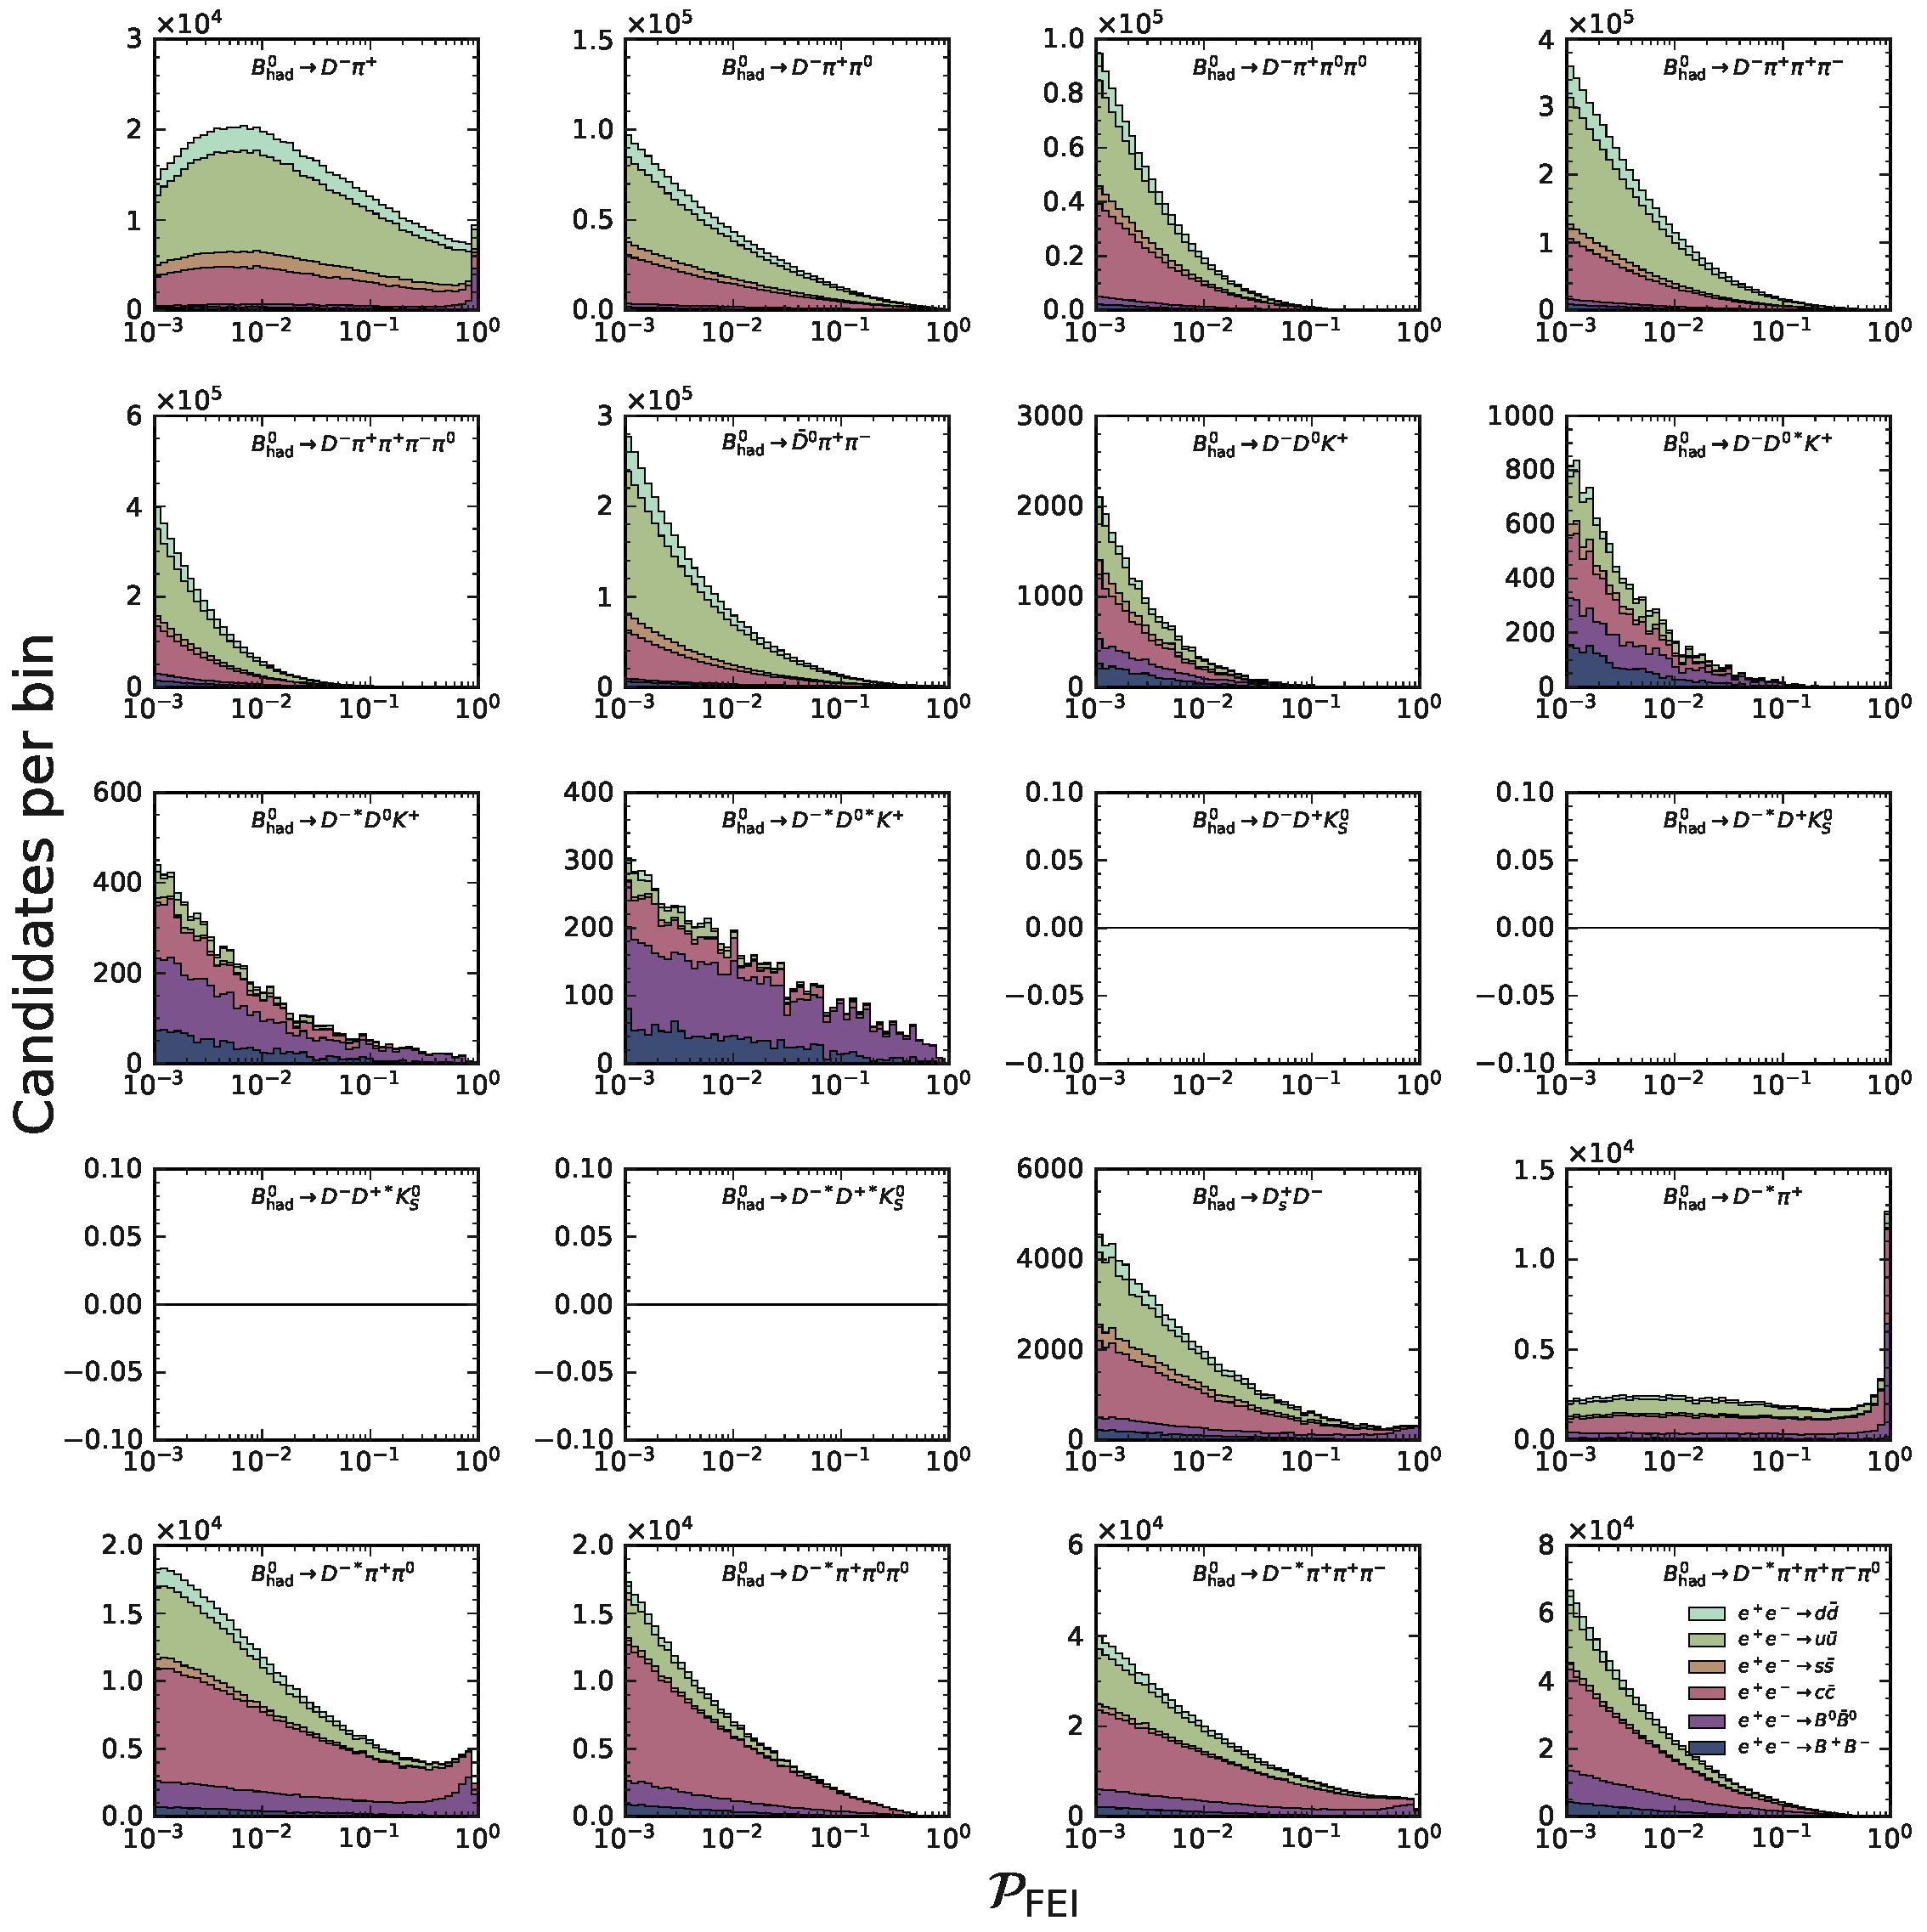
\includegraphics[width=1\textwidth]{figures/appendices/FEI_signal_probabilities/Bz_feiSigProbs1.pdf}

    \caption{\label{fig:feisigprobs3} \FEI signal probabilities for specific modes of \Bz reconstruction after requirements described in \Cref{sec:event_reconstruction}.
    This shows the signal probabilities for the first 20 \Bz modes in \Cref{tab:fei_modes}.
    Some figures are empty because no modes are reconstructed in those channels (either due to insufficient statistics, or no training available for said modes.)
    The legend, y and x axes are shared among all plots.
    }
\end{figure}

\begin{figure}[htbp!]

    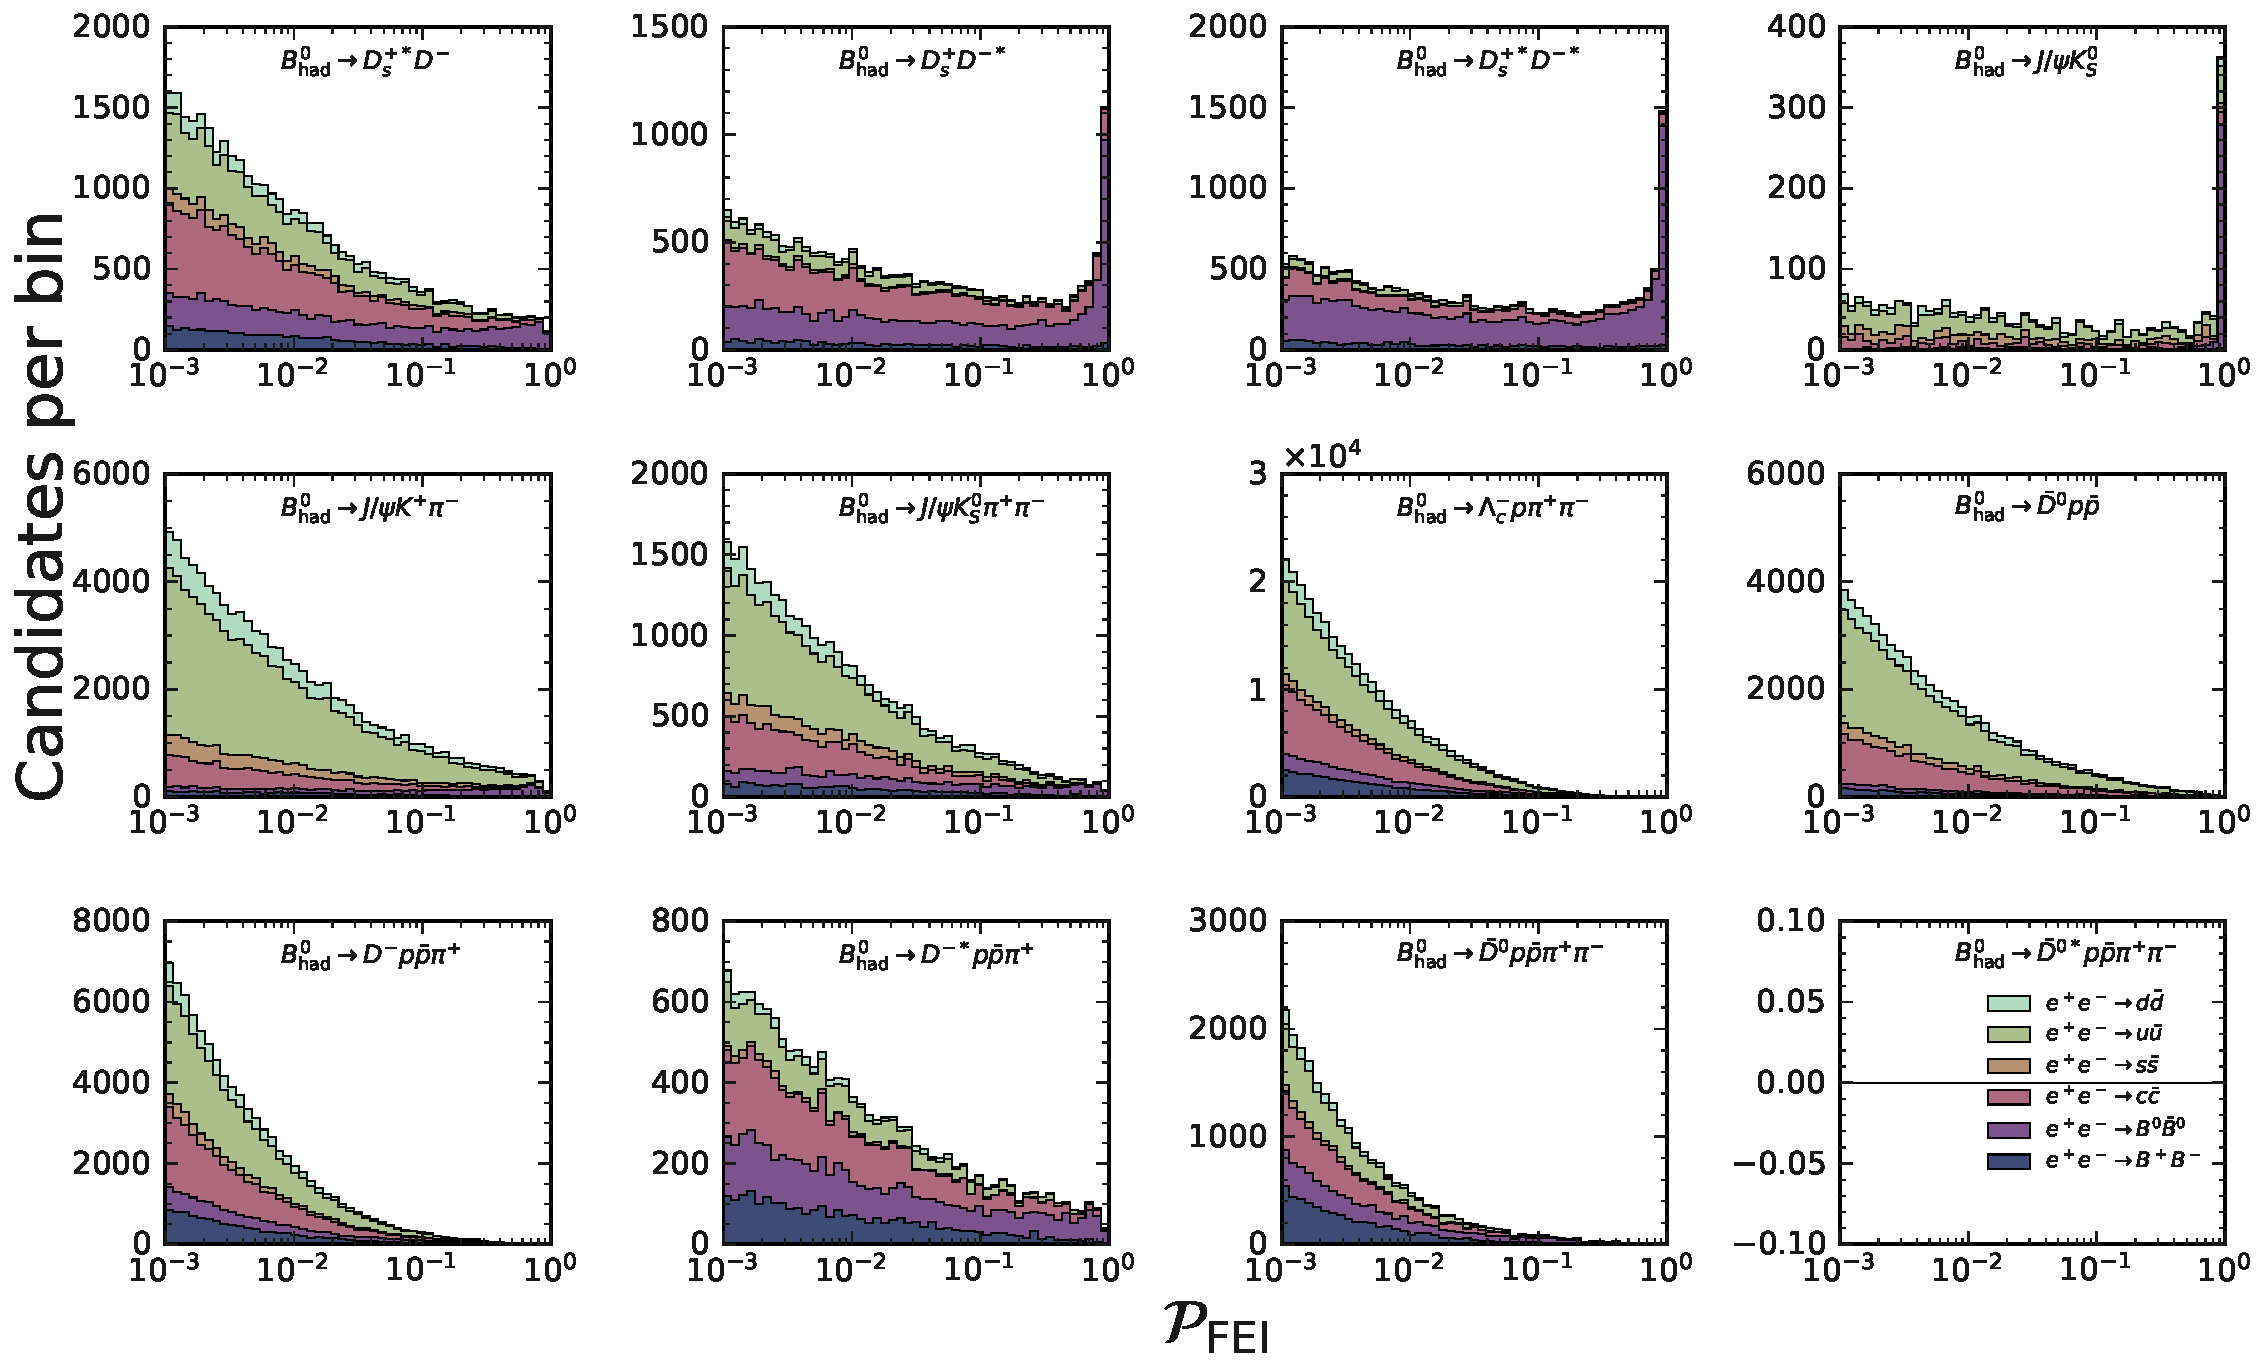
\includegraphics[width=1\textwidth]{figures/appendices/FEI_signal_probabilities/Bz_feiSigProbs2.pdf}

    \caption{\label{fig:feisigprobs4} \FEI signal probabilities for specific modes of \Bz reconstruction after requirements described in \Cref{sec:event_reconstruction}.
    This shows the signal probabilities for the modes 20-32 \Bz modes in \Cref{tab:fei_modes}.
    Some figures are empty because no modes are reconstructed in those channels (either due to insufficient statistics, or no training available for said modes.)
    The legend, y and x axes are shared among all plots.
    }
\end{figure}